\documentclass[unicode,12pt,aspectratio=169]{beamer}% 'unicode'が必要
\usepackage{luatexja}%これがないと日本語が出ない
%\documentclass[landscape]{ltjsarticle}
\usebackgroundtemplate{
\includegraphics[width=\paperwidth]{wao/md1.pdf}}
\usefonttheme{professionalfonts}
\setbeamertemplate{navigation symbols}{}
\usepackage{lmodern}
\usepackage{xcolor}

\begin{document}
\color{white}
あ

\begin{frame}
 \begin{center}
  \fontsize{35pt}{0pt}\selectfont 平方完成\\
  \fontsize{55pt}{0cm}\selectfont $y=2x^2-4x+1$  
 \end{center}

\end{frame}
\usebackgroundtemplate{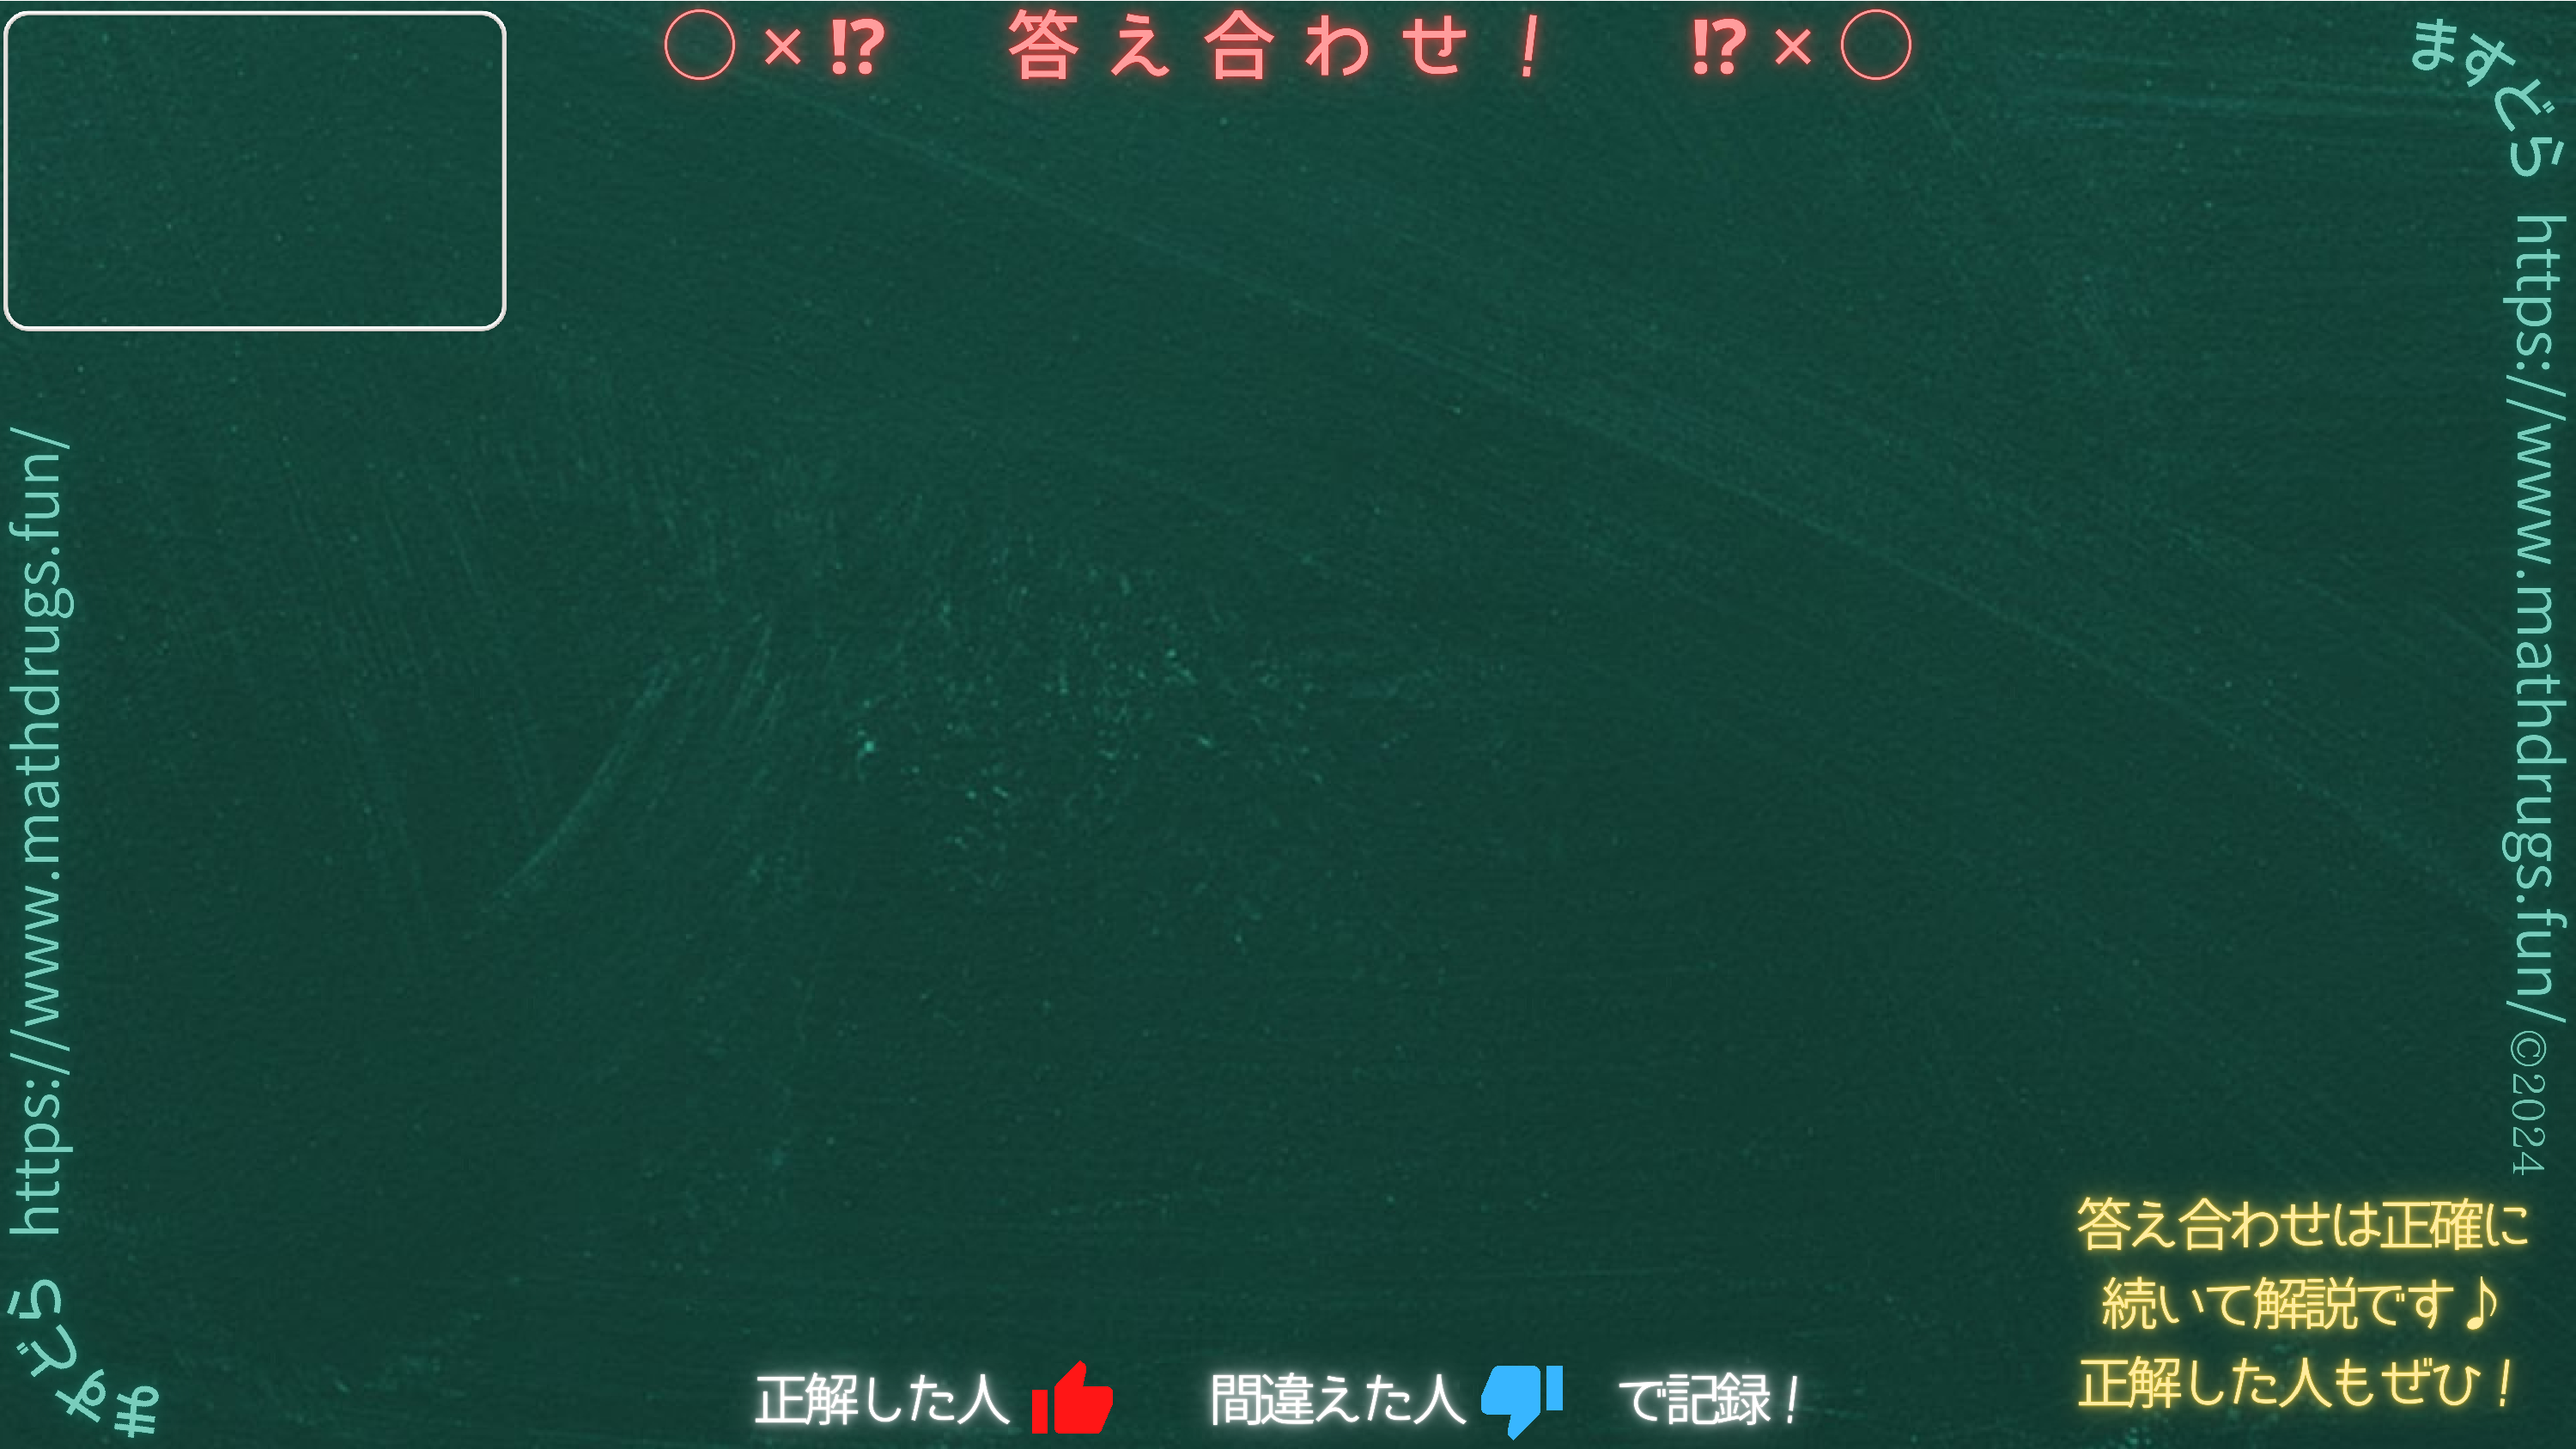
\includegraphics[width=\paperwidth]{md2.pdf}}
\begin{frame}
 wai
\end{frame}
\end{document}